\section{Study1: Observation on the stress-relieving ability of school scheduled uplift events}

\subsection{Sample}
We built our dataset based on two sources: 1) the microblogs of students coming from Taicang High School,
collected from January 1st, 2012 to February 1st, 2015;
and 2) list of scheduled school events, with exact start and end time.
We filtered out 124 active students according to their posting frequency from over 500 students,
and collected their microblogs throughout the whole high school career. Totally 29,232 microblogs are collected in this research,
where 236 microblogs per student on average, 1,387 microblogs maximally and 104 posts minimally.

\emph{Uplift events and stressor events}.
The list of weekly scheduled school events (from February 1st, 2012 to August 1st 2017) are collected from the school's official website
\footnote{http://stg.tcedu.com.cn/col/col82722/index.html}, with detailed event description and grade involved in the event.
There are 122 stressor events and 75 uplift events in total.
Here we give the examples of scheduled uplift and stressor events in high school life, as shown in Table~\ref{tab:example}.
There are 2-3 stressor events and 1-2 uplift event scheduled per month.

\begin{table}[H]
\caption{\small{Examples of school scheduled uplifts and stressor events.}}
\label{tab:example}
\resizebox{.45\textwidth}{9mm}{
\small{
\begin{tabular}{cccc}
\toprule
Type & Date	& Content	& Grade	\\
\midrule
\emph{stressor event} & 2014/4/16 & \emph{first day of mid-term exam} & grade1,2\\
\emph{uplift event} & 2014/11/5 & \emph{campus art festival} & grade1,2,3\\
\bottomrule
\end{tabular}
}
}
\end{table}

\emph{Stress detected from microblogs}.
Since our target is to observe the restoring impact of uplift events for teenagers under stress.
Based on previous research~\cite{XueUbicomp13},
we detected the stress level (ranging from 0 to 5) for each post;
and for each student, we aggregated the stress during each day by calculating the average stress of all posts.
The positive level (0-5) of each post is identified based on the frequency of positive words (see Section 5 for details).
Figure~\ref{fig:example} shows three examples of a student's stress fluctuation during three mid-term exams,
where the uplift event \emph{campus art festival} was scheduled ahead of the first exam,
the uplift event \emph{holiday} happened after the second exam,
and no scheduled uplift event was found nearby the third exam.
The current student exhibited differently in above three situations, with the stress lasting for different length and with different intensity.
\begin{figure}
\centering
\caption{Examples of school related stressor events, uplift events and a student's stress fluctuation}
\includegraphics[width=\linewidth]{figs/exampleWave.eps}
\label{fig:example}
\end{figure}


To further observe the influence of uplift events for students facing stressor events,
we statistic all the stressful intervals~\cite{Li2017Analyzing} detected surround the scheduled examinations over the 124 students during their high school career.
For each student, we divide all his/her stressful intervals into two sets:
1) stressful intervals under the influence of neighbouring uplift events (e.g., \emph{Halloween activity}), and 2) independent stressful intervals.
Figure~\ref{fig:frequency} shows five measures of each student during the above two conditions:
the \emph{accumulated stress}, the \emph{average stress} (per day), the \emph{length of stressful intervals},
the \emph{frequency of academic topic words}, and the \emph{ratio of academic stress among all types of stress}.
For each measure, we calculate the average value over all eligible slides for each student.

\begin{figure}
\centering
\caption{Compare students' stress during exam intervals in two situations:
1) affected by neighboring uplift events (U-SI), 2) no uplift events occurred nearby (SI)}
\includegraphics[width=\linewidth]{figs/frequency.eps}
\label{fig:frequency}
\end{figure}

\subsection{Findings}
Comparing each measure in scheduled exam slides under the two situations: 1) existing neighbouring uplift events or 2) no neighbouring scheduled uplift events,
we find that students during exams with neighbouring uplift events exhibit less average stress intensity (both on accumulated stress and average stress),
and the length of stress slides are relatively shorter.
%H1: stress length��intensity�½�

Further, we statistic the frequency of academic related topic words for each exam slide (as listed in Table \ref{tab:studyWords}),
and look into the ratio of academic stress among all five types of stress.
Results in Figure~\ref{fig:frequency} shows that most students talked less about the upcoming or just-finished exams when uplift events happened nearby,
with lower frequency and lower ratio.
%H1-3��
%The stress intensity and type distribution detected from each student's microblogs varies due to personal life experience, posting habits and express styles.
%modify1: ������仰������
The statistic result shows clues about the stress-relieving ability of scheduled uplift events,
and thus helps shape our problem as how to quantify the influence of uplift events,
thus to provide further guidance for planning campus activities to help relive students' stress effectively.
%\begin{figure}
%\centering
%\caption{Compare students' stress during exam intervals in two situations:
%1) affected by neighboring uplift events (U-SI), 2) no uplift events occurred nearby (SI)}
%\includegraphics[width=\linewidth]{figs/frequency.eps}
%\label{fig:frequency}
%\end{figure}

\begin{table}[h]
\centering
\caption{\small{Examples of academic related topic words.}}
\label{tab:studyWords}
\small{
\begin{tabular}{c}
\toprule
exam, fail, review, score, grade, test paper, rank, pass, math, chemistry\\
homework, recite, regress, fall behind, tension, stressed out, physics,\\
nervous, mistake, answer, question, puzzle, difficult, lesson, careless\\
\bottomrule
\end{tabular}
}
\end{table}

